\chapter{Result and Output}

\section{Result and Discussion}

The designed system is embedded in the model that emulates a traffic signal and the system is run by dumping the code in the RPi and running the python code. Once the system starts up, it by default enters the SMART mode and the traffic/congestion of each lane is measured and the corresponding time for which the green signal is to be turned ON is estimated depending upon the distance measured and the lane is turned on for the same amount of time. Then, it is switched to the next lane and the same process is repeated once again and then switches to the next lane and so on in a cyclic manner.

Also, the system listens continuously in background, for any update in the cloud for lane overriding which proves useful in case of emergencies. This data is updated and controlled using an android application that controls which lane is to be overridden or whether this feature in itself is to be turned on/off. It is secured using a login-based access, which authenticates only the personnel who has the proper rights to do so. To use this app to control the signal, one has to 1st login to the app by providing proper credentials and then select the lane which is to be turned ON and overridden. This data is stored in the backed powered by Ubidots, which is then sent to the RPi that is controlling the signal, which then takes the corresponding action to override that lane and turns it ON till further notice is received from the cloud (Ubidots) to turn it off, which is again done through the android application.

The system also can be toggled into NORMAL mode and back to SMART mode at any time using the toggle switch by traffic controller at the signal. It also has a reset switch that can be used by the traffic controller to completely reset the system in case of any errors.

\section{Output}

The output of the system running and it being controlled using the android application is documented. The following are the pictures that demonstrate the working of the system and it’s interaction with the cloud and the android application,

\begin{figure}[h]\centering
	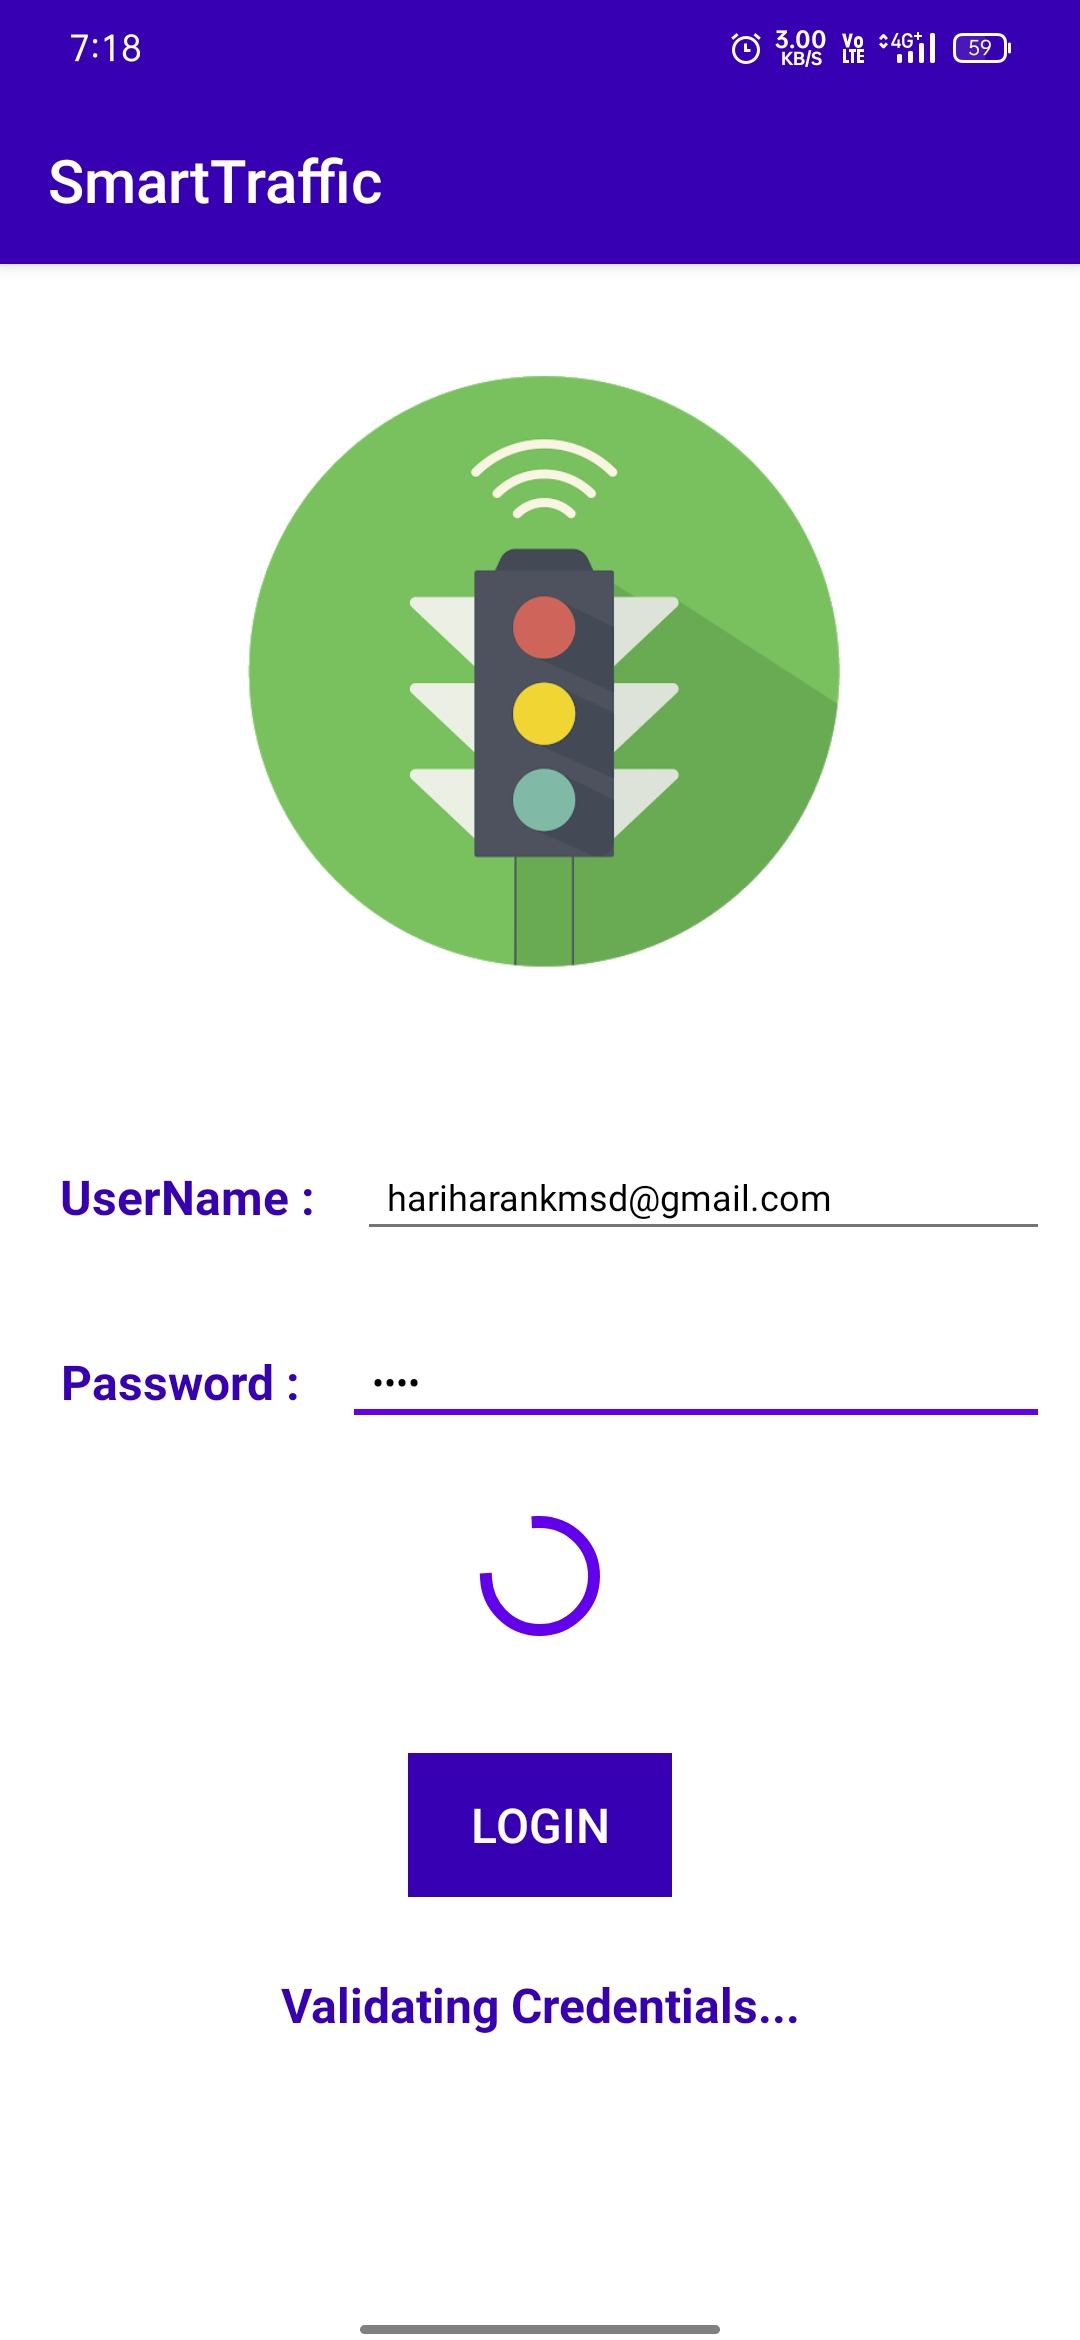
\includegraphics[width=1.75in]{./images/Login1.jpg}
        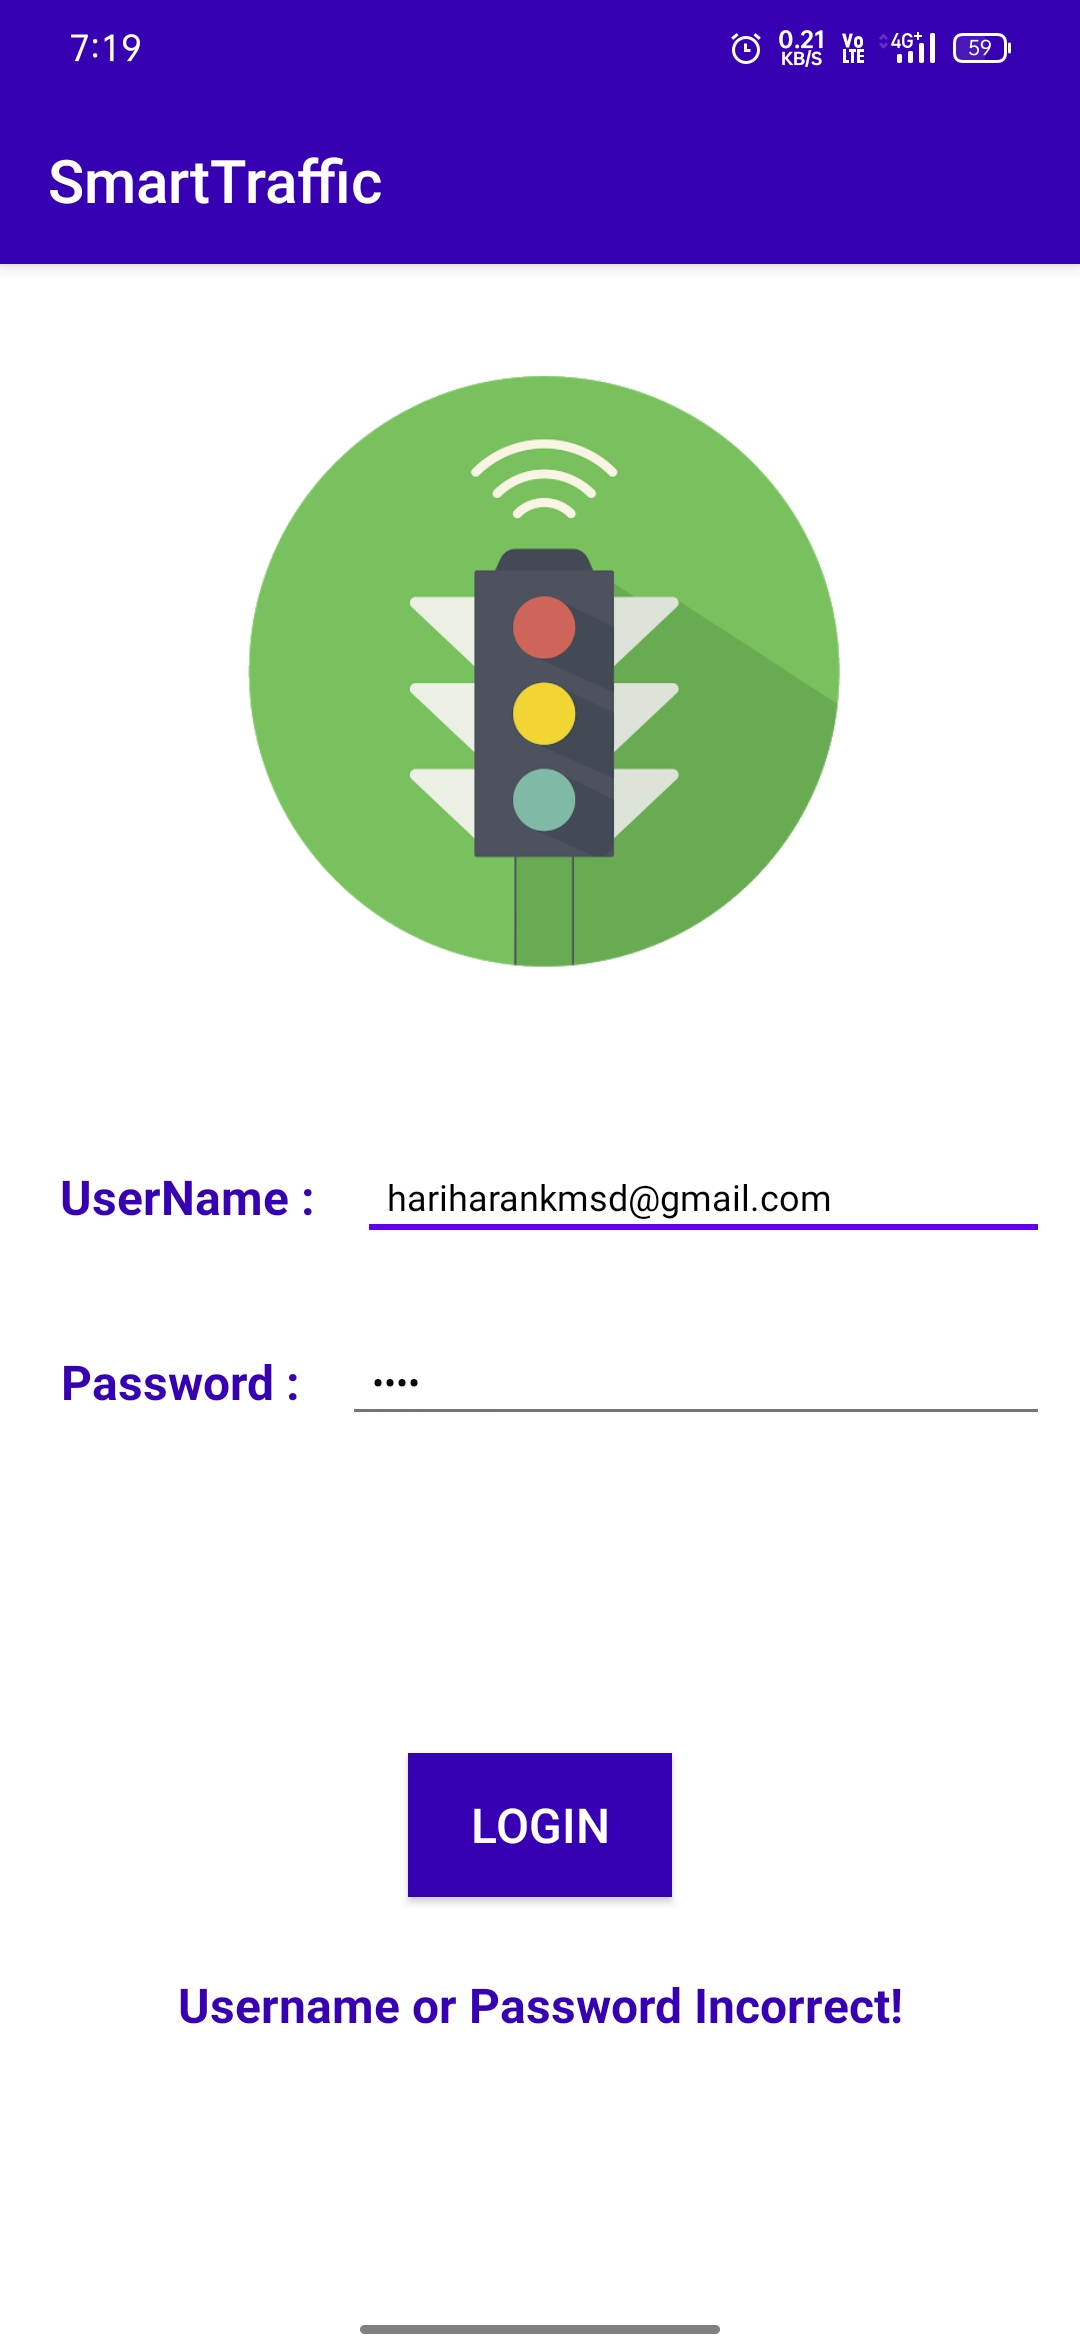
\includegraphics[width=1.75in]{./images/Login2.jpg}
        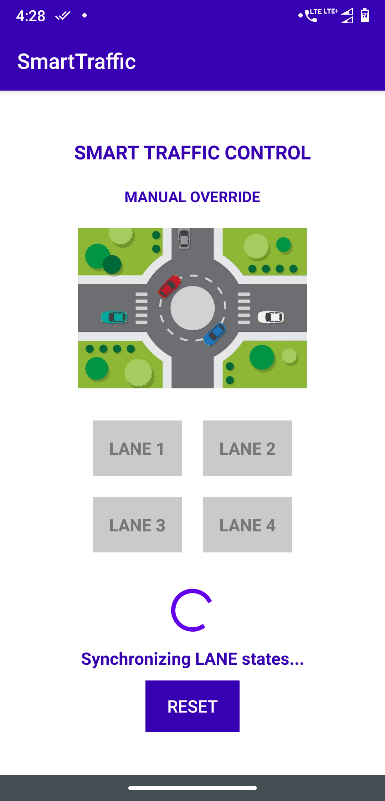
\includegraphics[width=1.75in]{./images/Login3.png}
	\caption{SmartTraffic Application - Login Interface}\label{Login}
\end{figure}

\pagebreak

\begin{figure}[h]\centering
	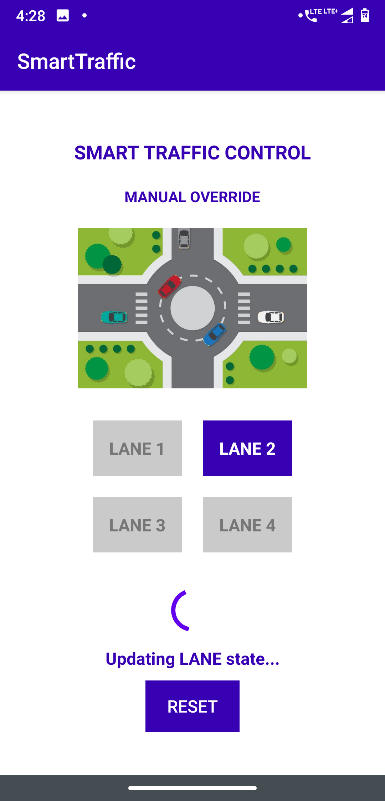
\includegraphics[width=1.75in]{./images/LaneOverride1.png}
        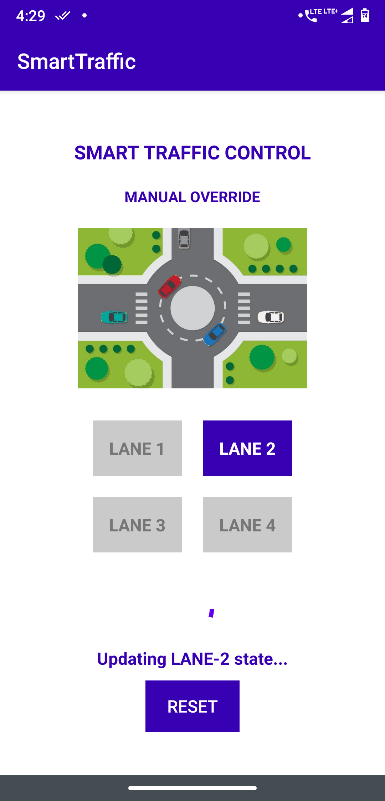
\includegraphics[width=1.75in]{./images/LaneOverride2.png}
        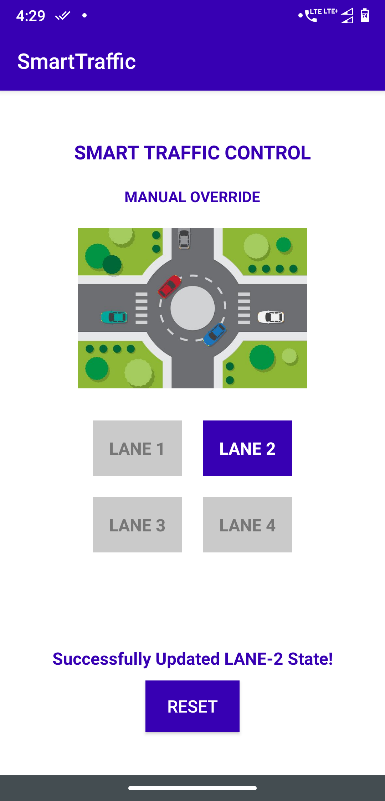
\includegraphics[width=1.75in]{./images/LaneOverride3.png}
	\caption{SmartTraffic Application - Lane Override}\label{LaneOverride}
\end{figure}

From above, we see that the android app covers following functionalities,

\begin{itemize}
    \item Login Authentication and Authorization
    \item Synchronizing the current override states of different lane states
    \item Overriding the lane state of any given lane to ON/OFF
    \item Resetting the Lane Override functionality
\end{itemize}